\documentclass{article}
%\usepackage{geometry}
\usepackage{enumitem}
%\usepackage{graphicx}

%\documentclass{article}
\usepackage{amsmath}
\usepackage{graphicx}
\usepackage{lipsum}  % For generating dummy text (remove in your actual document)
\usepackage[a4paper, margin=2.5cm]{geometry} % Specify A4 paper size and margins
\usepackage{draftwatermark}
% Define the watermark content, color, and position
\usepackage{xcolor}

\definecolor{lightgray}{rgb}{0.9,0.9,0.9}

\SetWatermarkText{MCT 517: Introduction: CNC, Robotics, and Automation (S.C. Nwafor}
\SetWatermarkScale{1}
\SetWatermarkColor{lightgray}
\SetWatermarkAngle{45}

\title{MCT 517: Introduction: CNC, Robotics, and Automation}
\author{Nwafor, Solomon Chibuzo\footnote{Department of Mechatronic Engineering, University of Nigeria, Nsukka.\\ Email: solomon.nwafor@unn.edu.ng}}
\date{October 24, 2023}


\begin{document}

\maketitle
\tableofcontents
\newpage

\section{CNC Machines}
\subsection{General Information about CNC Machines}
\begin{itemize}
    \item What is CNC machining?
    \item Types of CNC machines
    \item Advantages and disadvantages of CNC machining
    \item Applications of CNC machining
\end{itemize}

\subsection{Introduction to CNC Machines in Relation to Automation and Robotics}
\subsubsection{What is CNC Machining?}
Computer numerical control (CNC) machining is a subtractive manufacturing process in which material is removed from a workpiece to produce the desired part. CNC machines are controlled by computer programs that contain instructions for the machine's movements. CNC machines are used in a wide variety of industries to produce parts with complex geometries and tight tolerances. Some common applications of CNC machining include: Aerospace, Automotive, Medical, Electronics, Mold making, Tool and die-making, Prototyping, Rapid manufacturing.

\subsubsection{Types of CNC Machines}
There are many different types of CNC machines, each designed for a specific type of machining operation. Some of the most common types of CNC machines include:
\begin{enumerate}
    \item CNC milling machines: Use rotating cutting tools to remove material from a workpiece.
    \item CNC turning machines: Rotate the workpiece while a cutting tool removes material.
    \item CNC drilling machines: Create holes in workpieces.
    \item CNC boring machines: Enlarge existing holes in workpieces.
    \item CNC grinding machines: Use abrasive wheels to remove material from workpieces.
    \item CNC engraving machines: Use rotating tools to create designs on workpieces.
    \item CNC waterjet cutting machines: Use high-pressure jets of water to cut through materials.
\end{enumerate}

\subsubsection{Advantages of CNC Machining}
CNC machining offers a number of advantages over traditional manufacturing methods, including:
\begin{enumerate}
    \item Accuracy and precision: Produce parts with very high accuracy and precision.
    \item Consistency: Produce identical parts over and over again.
    \item Repeatability: Be reprogrammed to produce different parts, which makes them very versatile.
    \item Productivity: Are very productive and can produce large quantities of parts in a short amount of time.
\end{enumerate}

\subsubsection{CNC Machines in Relation to Automation and Robotics}
CNC machines can be integrated into automated and robotic manufacturing systems. In an automated manufacturing system, CNC machines are connected to other automated equipment, such as conveyors and material handling systems. This allows for the production of parts with minimal human intervention. In a robotic manufacturing system, CNC machines are equipped with robots that can perform tasks such as loading and unloading workpieces, changing tools, and measuring parts. This further increases the level of automation and can help to improve productivity and quality.

\subsubsection{Benefits of Integrating CNC Machines with Automation and Robotics}
There are a number of benefits to integrating CNC machines with automation and robotics, including:
\begin{enumerate}
    \item Increased productivity: Automated and robotic manufacturing systems can produce parts much faster than manual systems.
    \item Improved quality: Automated and robotic manufacturing systems can help to reduce errors and improve the overall quality of the finished product.
    \item Reduced costs: Automated and robotic manufacturing systems can help to reduce labor costs and other overhead expenses.
    \item Improved safety: Automated and robotic manufacturing systems can help to improve safety by reducing the need for human workers to interact with dangerous machinery.
\end{enumerate}

CNC machines are powerful tools that can be used to produce a wide variety of parts with high accuracy and precision. Integrating CNC machines with automation and robotics can further increase productivity, quality, and safety.

\newpage

\section{Lecture Material on Operation of CNC Machines}
\subsection{CNC Machine Components}
CNC machines are made up of a number of different components, including:
\begin{itemize}
    \item Machine tool: This is the physical machine that performs the machining operations.
    \item CNC control unit: This is the computer that controls the machine tool.
    \item Servo drives and motors: These components drive the machine tool's axes and spindle.
    \item Sensors: These components provide feedback to the CNC control unit.
    \item Tool changer: This component automatically loads and unloads tools from the machine tool.
    \item Workpiece fixture: This component holds the workpiece in place during machining.
\end{itemize}

\subsection{Setting up a CNC Machine}
Setting up a CNC machine involves several steps, including:
\begin{enumerate}
    \item Preparing the workpiece: Ensure that the workpiece is clean and free from any burrs or sharp edges.
    \item Fixturing the workpiece: Secure the workpiece in the workpiece fixture.
    \item Selecting and loading the tools: Choose the appropriate tools for the job and load them into the tool changer.
    \item Setting the work and tool offsets: This involves setting the starting point for the machining operations and ensuring that the tools are at the correct height.
    \item Running a test program: This involves running a test program to ensure that everything is set up correctly and that there are no collisions.
\end{enumerate}

\subsection{Operating a CNC Machine}
Operating a CNC machine involves:
\begin{enumerate}
    \item Loading the CNC program: This is the program that contains the instructions for the machining operations.
    \item Setting the machine parameters: This includes setting the spindle speed, feed rate, and other machine settings.
    \item Starting the machining process: This involves pressing the start button to begin the machining operations.
    \item Monitoring the machining process: This involves watching the machine to ensure that everything is running smoothly and that there are no problems.
    \item Unloading the finished part: Once the machining operations are complete, unload the finished part from the machine.
\end{enumerate}

\subsection{Maintenance of CNC Machines}
Regular maintenance is crucial for ensuring the long life and high performance of CNC machines. Maintenance tasks include:
\begin{enumerate}
    \item Cleaning the machine: Regularly clean the machine to remove chips, coolant, and other debris.
    \item Lubricating the machine: Ensure that all moving parts are properly lubricated.
    \item Checking the alignment: Regularly check and adjust the alignment of the machine to ensure accuracy.
    \item Replacing worn parts: Replace any parts that are worn or damaged.
    \item Calibrating the machine: Regularly calibrate the machine to ensure accuracy.
\end{enumerate}

\subsection{Troubleshooting CNC Machines}
When problems occur, it is important to troubleshoot the CNC machine to determine the cause and find a solution. Some common problems and their solutions include:
\begin{enumerate}
    \item Machine not starting: Check the power supply, fuses, and emergency stop button.
    \item Poor surface finish: Check the tool condition, cutting parameters, and workpiece material.
    \item Inaccurate parts: Check the machine calibration, tool length offset, and workpiece setup.
    \item Machine making strange noises: Check for loose parts, tool condition, and proper lubrication.
    \item Machine crashing: Check the CNC program for errors, tool setup, and workpiece setup.
\end{enumerate}

\section*{Practical Application of Tool Wear Offset, Feed Function, and Spindle Function in Automation and Robotics}

\subsection*{Tool Wear Offset}

\subsubsection*{What is tool wear offset?}
Tool wear offset is a parameter in a CNC machine that compensates for the gradual wear of cutting tools. As tools are used, they become smaller and duller, which can affect the accuracy of the finished parts. Tool wear offset allows the CNC machine to adjust the position of the tool to compensate for this wear, ensuring that parts are produced to the correct dimensions.

\subsubsection*{How to use tool wear offset to maintain part accuracy}
To use tool wear offset to maintain part accuracy, you must first measure the amount of wear on the cutting tool. This can be done using a variety of methods, such as a tool microscope or a cutting force sensor. Once you have measured the wear, you can enter this value into the tool wear offset parameter in the CNC machine.

The CNC machine will then use this value to adjust the position of the tool to compensate for the wear. For example, if the tool has worn by 0.1mm, the CNC machine will move the tool 0.1mm closer to the workpiece. This ensures that the finished part will be produced to the correct dimensions, even as the tool wears down.

\subsubsection*{Practical applications}
Tool wear offset is used in a wide variety of automation and robotics applications, including:
\begin{itemize}
    \item CNC machining: Tool wear offset is essential for maintaining part accuracy in CNC machining.
    \item Robotic welding: Tool wear offset can be used to compensate for the wear of welding electrodes, ensuring that welds are of consistent quality.
    \item Automated assembly: Tool wear offset can be used to compensate for the wear of assembly tools, ensuring that parts are assembled correctly.
\end{itemize}

\subsection*{Feed Function}

\subsubsection*{What is feed function?}
The feed function in a CNC machine controls the rate at which the tool moves relative to the workpiece. The feed rate is typically measured in millimeters per minute (mm/min).

\subsubsection*{How to select the correct feed rate for different materials and operations}
The correct feed rate to use depends on a number of factors, including the material being machined, the type of operation being performed, and the desired surface finish.

For example:
\begin{itemize}
    \item Harder materials generally require slower feed rates than softer materials.
    \item Roughing operations can use faster feed rates than finishing operations.
    \item A smoother surface finish can be achieved using slower feed rates.
\end{itemize}

\subsubsection*{Practical applications}
The feed function is used in a wide variety of automation and robotics applications, including:
\begin{itemize}
    \item CNC machining: The feed function is essential for controlling the machining process and producing parts with the desired finish.
    \item Robotic painting: The feed function can be used to control the speed at which a robot moves a paint sprayer, ensuring that a consistent coat of paint is applied.
    \item Automated packaging: The feed function can be used to control the speed at which a robot moves products along a conveyor belt, ensuring that they are packaged correctly.
\end{itemize}

\subsection*{Spindle Function}

\subsubsection*{What is spindle function?}
The spindle function in a CNC machine controls the rotation of the spindle. The spindle speed is typically measured in revolutions per minute (RPM).

\subsubsection*{How to use spindle functions such as threading and tapping}
The spindle function can be used to perform a variety of operations, including threading and tapping.

Threading is the process of cutting a helical groove into a workpiece. To thread a workpiece, the spindle is rotated while the tool is fed into the workpiece. The feed rate and spindle speed must be carefully coordinated to ensure that the correct thread pitch is produced.

Tapping is the process of creating a threaded hole in a workpiece. To tap a hole, the spindle is rotated while the tap is fed into the hole. The feed rate and spindle speed must be carefully coordinated to ensure that the tap does not break.

\subsubsection*{Practical applications}
The spindle function is used in a wide variety of automation and robotics applications, including:
\begin{itemize}
    \item CNC machining: The spindle function is essential for machining a variety of features, such as holes, threads, and contours.
    \item Robotic assembly: The spindle function can be used to control the rotation of tools such as screwdrivers and nut runners, ensuring that screws and nuts are tightened to the correct torque.
    \item Automated inspection: The spindle function can be used to rotate workpieces while they are being inspected, ensuring that all surfaces are inspected thoroughly.
\end{itemize}

\subsubsection*{Source references}
\begin{itemize}
    \item CNC Programming for Machining and Manufacturing: Concepts, Applications, and Programming by Mark J. Petro
    \item Robotics and Manufacturing Automation by Joseph F. Engelberger
    \item Automated Manufacturing Systems by James A.
\end{itemize}

\section*{Programming of CNC in absolute and incremental systems}

\subsection*{Absolute and incremental programming coordinates}
There are two ways to program the coordinates of a CNC machine: absolute and incremental.

Absolute programming specifies the final position of the tool in each axis. This is done by specifying the X, Y, and Z coordinates of that position relative to a fixed origin, usually the machine origin or a work offset. For example, the G-code G0 X100 Y100 Z50 would move the tool to the position X=100, Y=100, and Z=50.

Incremental programming specifies the distance that the tool should move in each axis from its current position. This is done by specifying the X, Y, and Z coordinates of the move in parentheses. For example, the G-code G1 X(50) Y(50) Z(50) would move the tool 50 units in the X, Y, and Z axes from its current position.

\subsection*{G-codes and M-codes}
G-codes and M-codes are the programming language that CNC machines use to understand what to do. G-codes are used to control the movement of the machine, such as G0 for rapid movement and G1 for linear interpolation. M-codes are used to control auxiliary functions, such as M3 for spindle start and M5 for spindle stop.

Here are some examples of common G-codes and M-codes:
\begin{itemize}
    \item G0 - Rapid movement
    \item G1 - Linear interpolation
    \item G2 - Circular interpolation clockwise
    \item G3 - Circular interpolation counterclockwise
    \item M3 - Spindle start
    \item M5 - Spindle stop
    \item M6 - Tool change
\end{itemize}

\subsection*{Practical application of G-codes and M-codes in CNC programming}
G-codes and M-codes are used to create CNC programs that control the movement and operation of the machine. A typical CNC program consists of a sequence of G-codes and M-codes that instruct the machine to perform specific operations.

For example, a CNC program to drill a hole in a workpiece may consist of the following sequence:
\begin{enumerate}
    \item G0 X0 Y0 Z50 (Move to the starting position)
    \item M6 T1 (Select tool 1)
    \item M3 S500 (Start the spindle at 500 RPM)
    \item G1 Z-10 F100 (Move the tool down to drill the hole at a feed rate of 100 mm/min)
    \item G0 Z50 (Retract the tool)
    \item M5 (Stop the spindle)
\end{enumerate}

This program will move the tool to the starting position, select the appropriate tool, start the spindle, drill the hole, retract the tool, and stop the spindle.

\subsection{CNC Programming Examples}
Given the diagram of a workpiece provided Figure 1, your task is to write the CNC code to machine the workpiece using a CNC milling machine. Utilize the absolute programming coordinate system.\\

\begin{figure}[h!]
\begin{center}
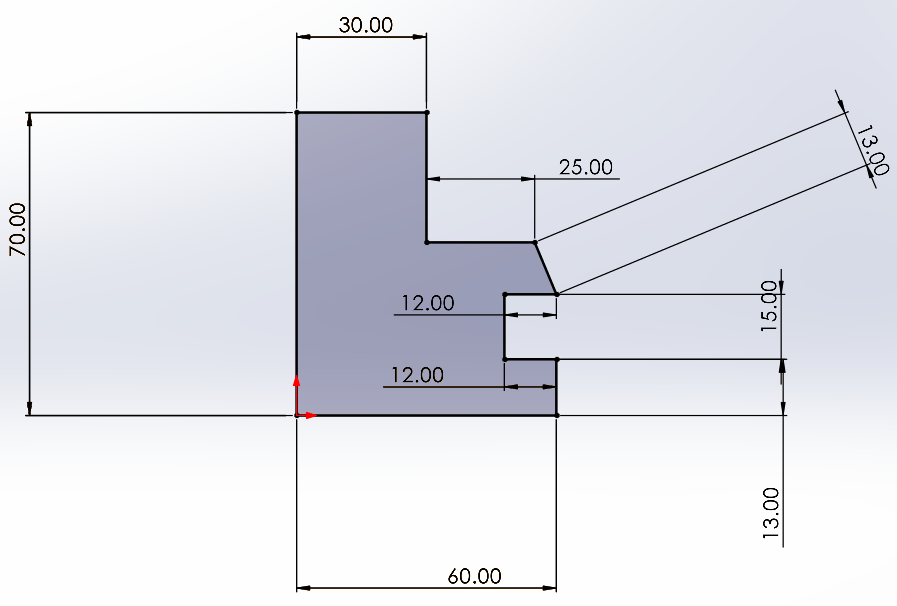
\includegraphics[width=10.0cm]{milling1}
\caption{CNC Milling Operation}
\label{fig1}
\end{center}
\end{figure}

Instructions:
\begin{enumerate}
	\item Assume you are starting at the origin point (0,0).
	\item Use a suitable tool for milling and mention the tool number in your code.
	\item Clearly define your tool path, starting and ending points.
	\item Make sure to use feed rates and spindle speeds appropriate for the material of the workpiece (you may specify a material or leave it to the student's discretion).
	\item Include all necessary safety and initialization commands to ensure the machine operates correctly.
	\item Ensure your code is properly formatted and commented for clarity.
\end{enumerate}

Based on the diagram, consider the following dimensions (all dimensions are in mm):
\begin{enumerate}
\item Overall length of the workpiece: 70.00
\item Overall width of the workpiece: 60.00
\item ...continue with other measurements as needed from the diagram
\end{enumerate}

Hint: Remember to use absolute coordinates (G90) when programming your tool path.

You are expected to provide a full CNC code, with initialization, tool selection, feed rates, and absolute coordinate moves that represent the machining of the provided workpiece diagram.\\

\textbf{Solution}\\
Begin the CNC programming
\begin{itemize}
\item G21 ; Set units to mm (can change to G20 for inches)
\item G90 ; Absolute positioning

\item M03 ; Start the spindle
\item G04 P2000 ; Wait for 2 seconds for the spindle to come up to speed

\item G00 Z5 ; Lift tool to a safe height of 5 units
\item G00 X0 Y0 ; Rapid move to origin

\item G01 Z-15 F100 ; Plunge tool to -15 units to make a cut of 10 mm at a feed rate of 100 units/min
\item \textbf{Begin cutting profile}
\item G01 X0 Y70 F300 ; Move vertically up to the top
\item G01 X30 Y70 ; Move horizontally to the right
\item G01 X30 Y40 ; Move downwards
\item G01 X55 Y40 ; Move horizontally to the right
\item G01 X60 Y28 ; Move vertically downwards to make the diagonal line
\item G01 X48 Y28 ; Move horizontally to the left
\item G01 X48 Y13 ; Move vertically downwards
\item G01 X60 Y13 ; Move horizontally to the left
\item G01 X60 Y0 ; Move upwards to the starting height
\item G01 X0 Y0 ; Return to origin

\item G00 Z15 ; Lift the tool up to a safe height

\item M05 ; Stop the spindle
\item M30 ; End of program

\end{itemize}
\maketitle
\textbf{Classwork}

Given the provided workpiece diagram in Figure 2, your assignment is to write the CNC programming required to machine the part using both milling and drilling operations.

\textbf{Instructions}

\begin{enumerate}
    \item Start your programming from the origin point (0,0).
    \item Use the absolute programming coordinate system.
    \item Choose a suitable tool for milling and drilling. Specify the tool number in your code.
    \item The tool is to go a depth of 10mm into the workpiece.
    \item The feed rate for all operations should be set to 200 mm/min.
    \item Clearly define your tool path, starting and ending points, including any tool changes.
    \item Use appropriate spindle speeds considering the material and operation type (you may specify a material or leave it to students' discretion).
    \item Make sure to incorporate safety and initialization commands to ensure correct machine operation.
    \item Comment your code for clarity, explaining each operation and any decisions made.
\end{enumerate}

Overall dimensions, hole positions, and other necessary measurements can be taken from the provided diagram.\\


\textbf{Hints}

\begin{itemize}
    \item Remember to use absolute coordinates (G90) when programming your tool path.
    \item When programming the drilling operation, consider the center positions of the holes and the required depth.
\end{itemize}

\textbf{Submission Details}

\begin{enumerate}
    \item Submit your completed CNC code in a text file.
    \item Along with the CNC code, submit a brief report explaining your tool path strategy, tool choices, and any challenges faced during the programming process.
\end{enumerate}

\textbf{Assessment Criteria}\\

\begin{enumerate}
    \item Correctness of the CNC code.
    \item Efficiency of the tool path.
    \item Clarity and organization of the code, including comments.
    \item Quality and depth of the explanation in the report.
\end{enumerate}


Wishing you the best in this task. Remember, understanding the process is just as important as the final output. Feel free to seek clarifications if any part of the assignment is unclear.

\begin{figure}[h!]
\begin{center}
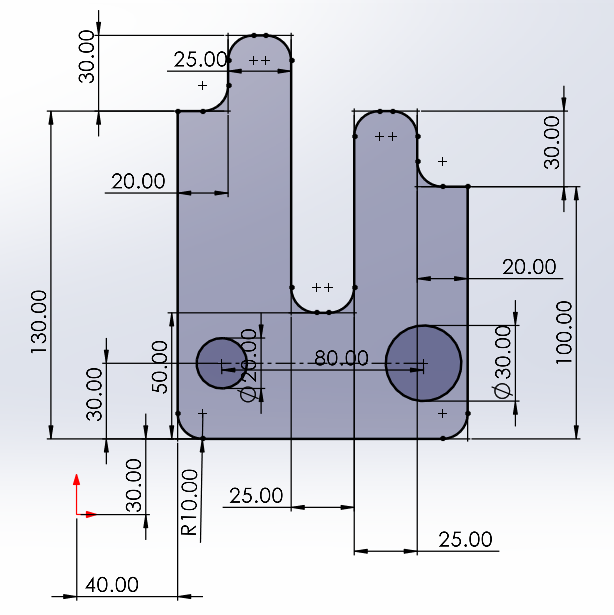
\includegraphics[width=10.0cm]{milling2}
\caption{CNC Milling Operation}
\label{fig2}
\end{center}
\end{figure}


\section*{Conclusion}

In automation and robotics, the understanding and application of tool wear offset, feed function, and spindle function are crucial for maintaining accuracy and efficiency in manufacturing processes. These functions, along with proper CNC programming in both absolute and incremental systems, enable the production of high-quality parts and products. With the combination of skilled operators and advanced CNC machines, industries can achieve optimal performance and productivity in their operations.\\

Operating and maintaining a CNC machine requires a solid understanding of its components, setup procedures, and operation. Regular maintenance and proper troubleshooting can help to ensure that the machine performs at its best and has a long service life.

\section*{Sources}
\begin{enumerate}
    \item CNC Programming Handbook: A Comprehensive Guide to Practical CNC Programming (2003) by Peter Smid
\end{enumerate}

\end{document}
